% !TeX root = RJwrapper.tex
\title{Connecting R with D3 for dynamic graphics, to explore multivariate data
with tours}
\author{by Michael Kipp, Dianne Cook, Ursula Laa}

\maketitle

\abstract{%
The tourr package in R has several algorithms and displays for showing
multivariate data as a sequence of low-dimensional projections. It can
display as a movie but has no capacity for interaction, such as stop/go,
change tour type, drop/add variables. The tourrGui package provides
these sorts of controls, but the interface is programmed with the dated
RGtk2 package. This work explores using custom messages to pass data
from R to D3 for viewing, using the Shiny framework.
}

\subsection{Introduction}\label{introduction}

The tour algorithm (Cook et al. \protect\hyperlink{ref-gt_pp}{1995};
Cook et al. \protect\hyperlink{ref-gt_pp_mc}{2007}) is a way of
systematically generating and displaying projections of high-dimensional
spaces in order for the viewer to examine the multivariate distribution
of data. It can do this either randomly, or by picking projections
judged interesting according to some criterion or index function. The
tourr package (Wickham et al. \protect\hyperlink{ref-tourr}{2011})
provides the computing and display in R (R Core Team
\protect\hyperlink{ref-R}{2018}; Ihaka and Gentleman
\protect\hyperlink{ref-ihaka:1996}{1996}) to make several types of
tours: grand, guided, little and local. The projection dimension can be
chosen between one and the number of variables in the data. The display,
though, has no capacity for interaction. The viewer can watch the tour
like a movie, but not pause it and restart, or change tour type, or
number of variables.

These interactive controls were provided with the tourrGui package
(Huang, Cook, and Wickham \protect\hyperlink{ref-tourrGui}{2012}), with
was programmed with the RGtk2 package (Lawrence and Temple Lang
\protect\hyperlink{ref-RGtk2}{2010}). This is not the toolkit of choice
today, and has been superceded with primarily web-capable tools, like
Shiny (Chang et al. \protect\hyperlink{ref-shiny}{2017}). To display
dynamic graphics though, is not straight-forward. This paper explains
how to use D3 (Bostock, Ogievetsky, and Heer
\protect\hyperlink{ref-D3}{2011}) as the display engine in a Shiny
graphical user interface (GUI), using custom message passing between
server and client.

\subsection{Creating a tour, with the tourr
package}\label{creating-a-tour-with-the-tourr-package}

The \pkg{tourr} package (Wickham et al.
\protect\hyperlink{ref-tourr}{2011}) is an R implementation of the tour
algorithms discussed in Cook et al.
(\protect\hyperlink{ref-gt_pp_mc}{2007}). It includes methods for
geodesic interpolation and basis generation, as well as an
implementation of the simulated annealing algorithm to optimise
projection pursuit indices for the guided tour. The tour can be
displayed directly in the R graphics device, for example:

\begin{Schunk}
\begin{Sinput}
library(tourr)
# quartz() # to display on a Mac
# X11() # For windows
# The Rstudio graphics device is not advised
animate_dist(flea[, 1:6], center = TRUE)
\end{Sinput}
\end{Schunk}

generating the animation, with some stills shown in Figure \ref{tour}.

\begin{figure}[ht]
\centerline{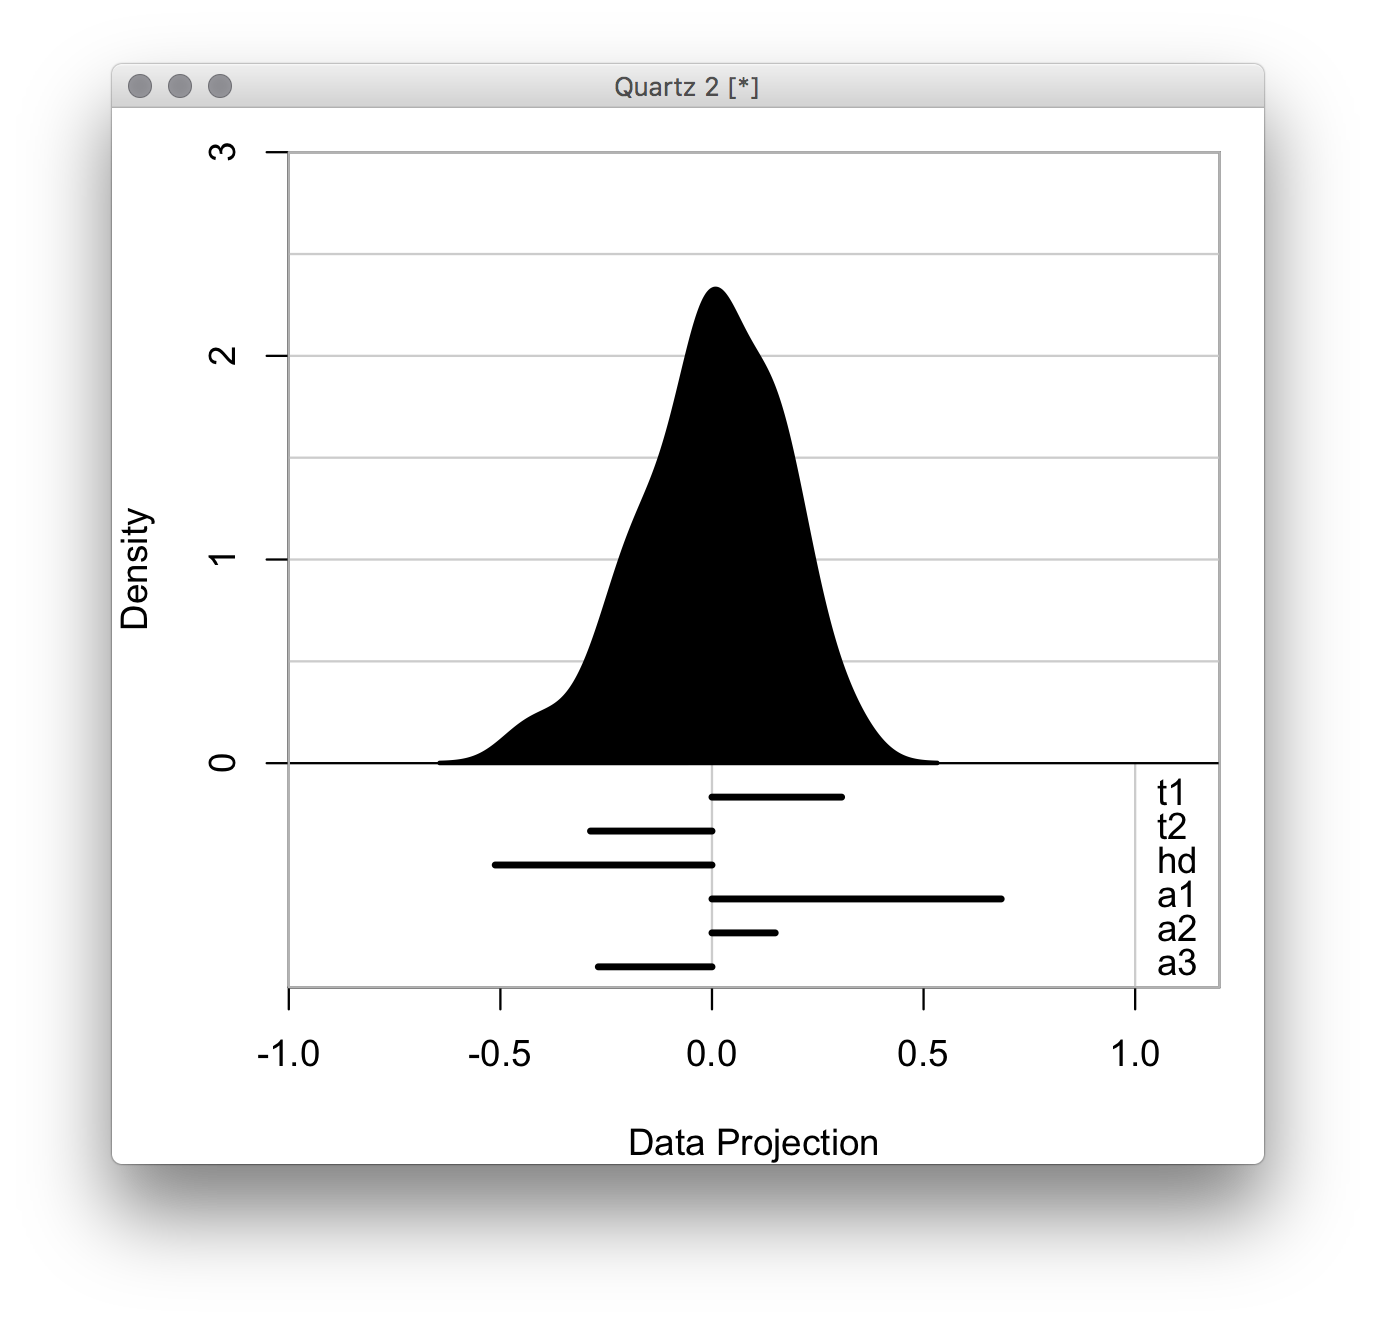
\includegraphics[width=5cm]{figures/tour1.png}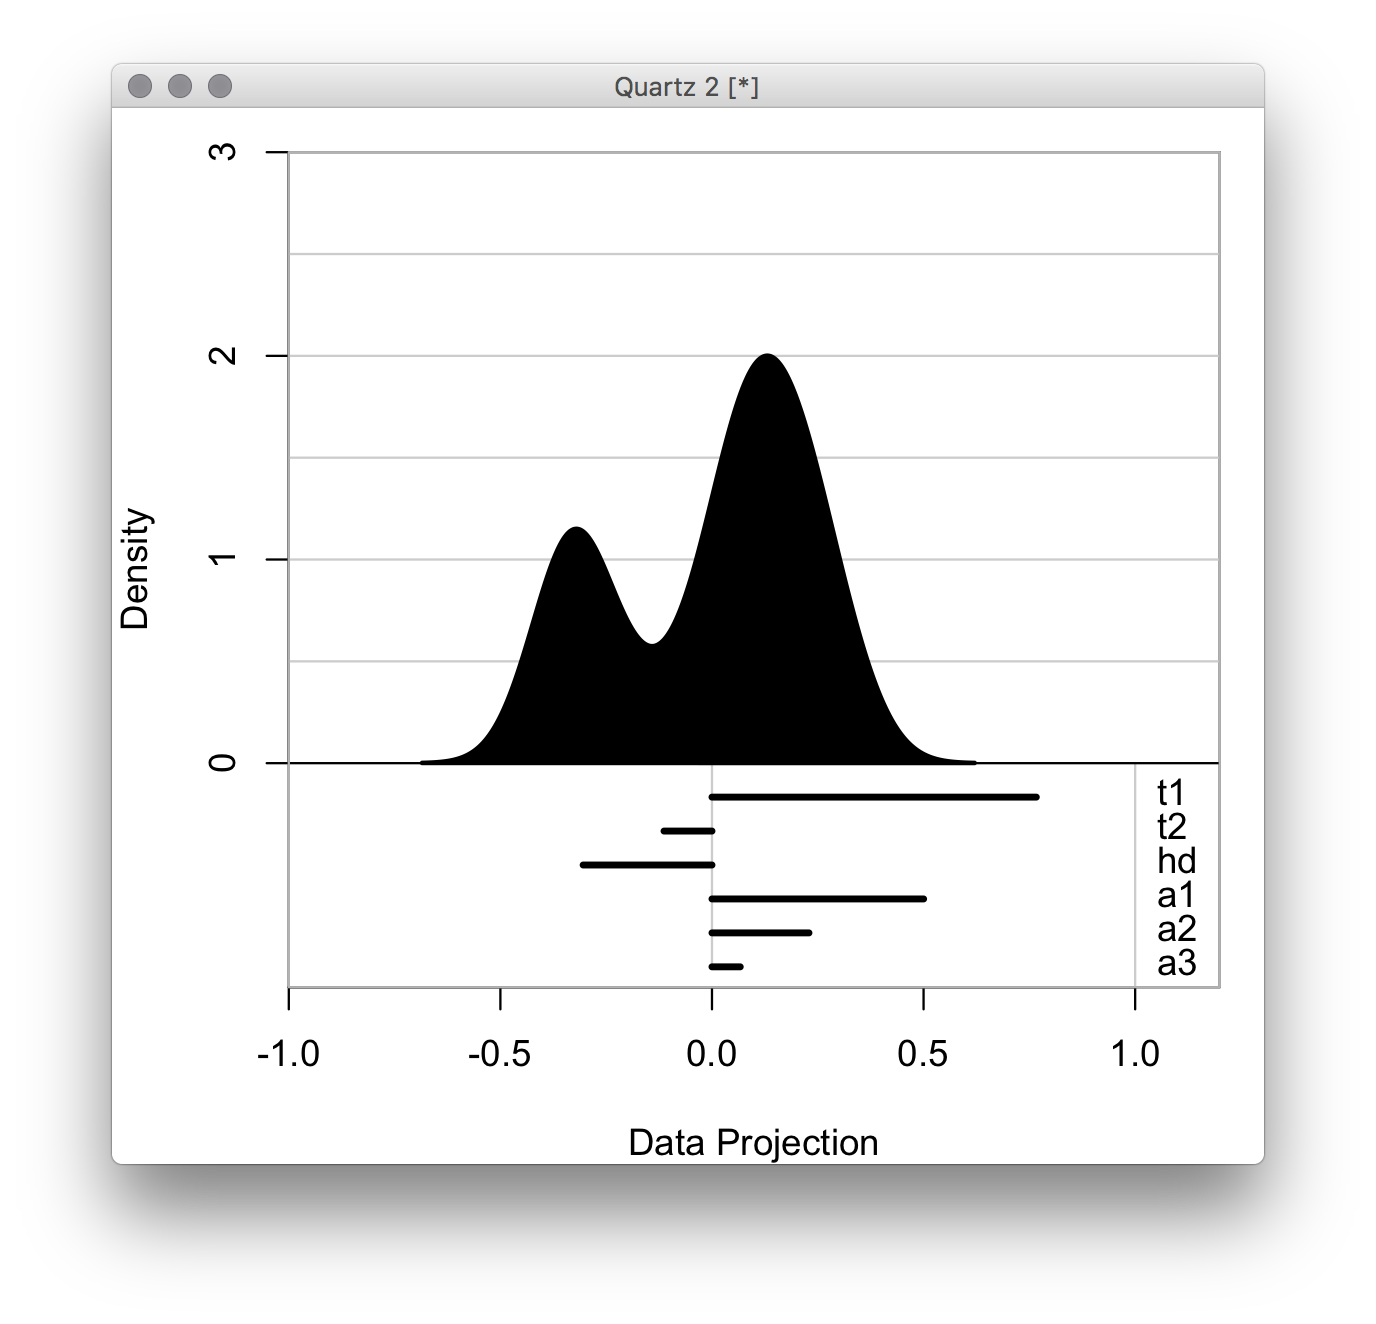
\includegraphics[width=5cm]{figures/tour2.png}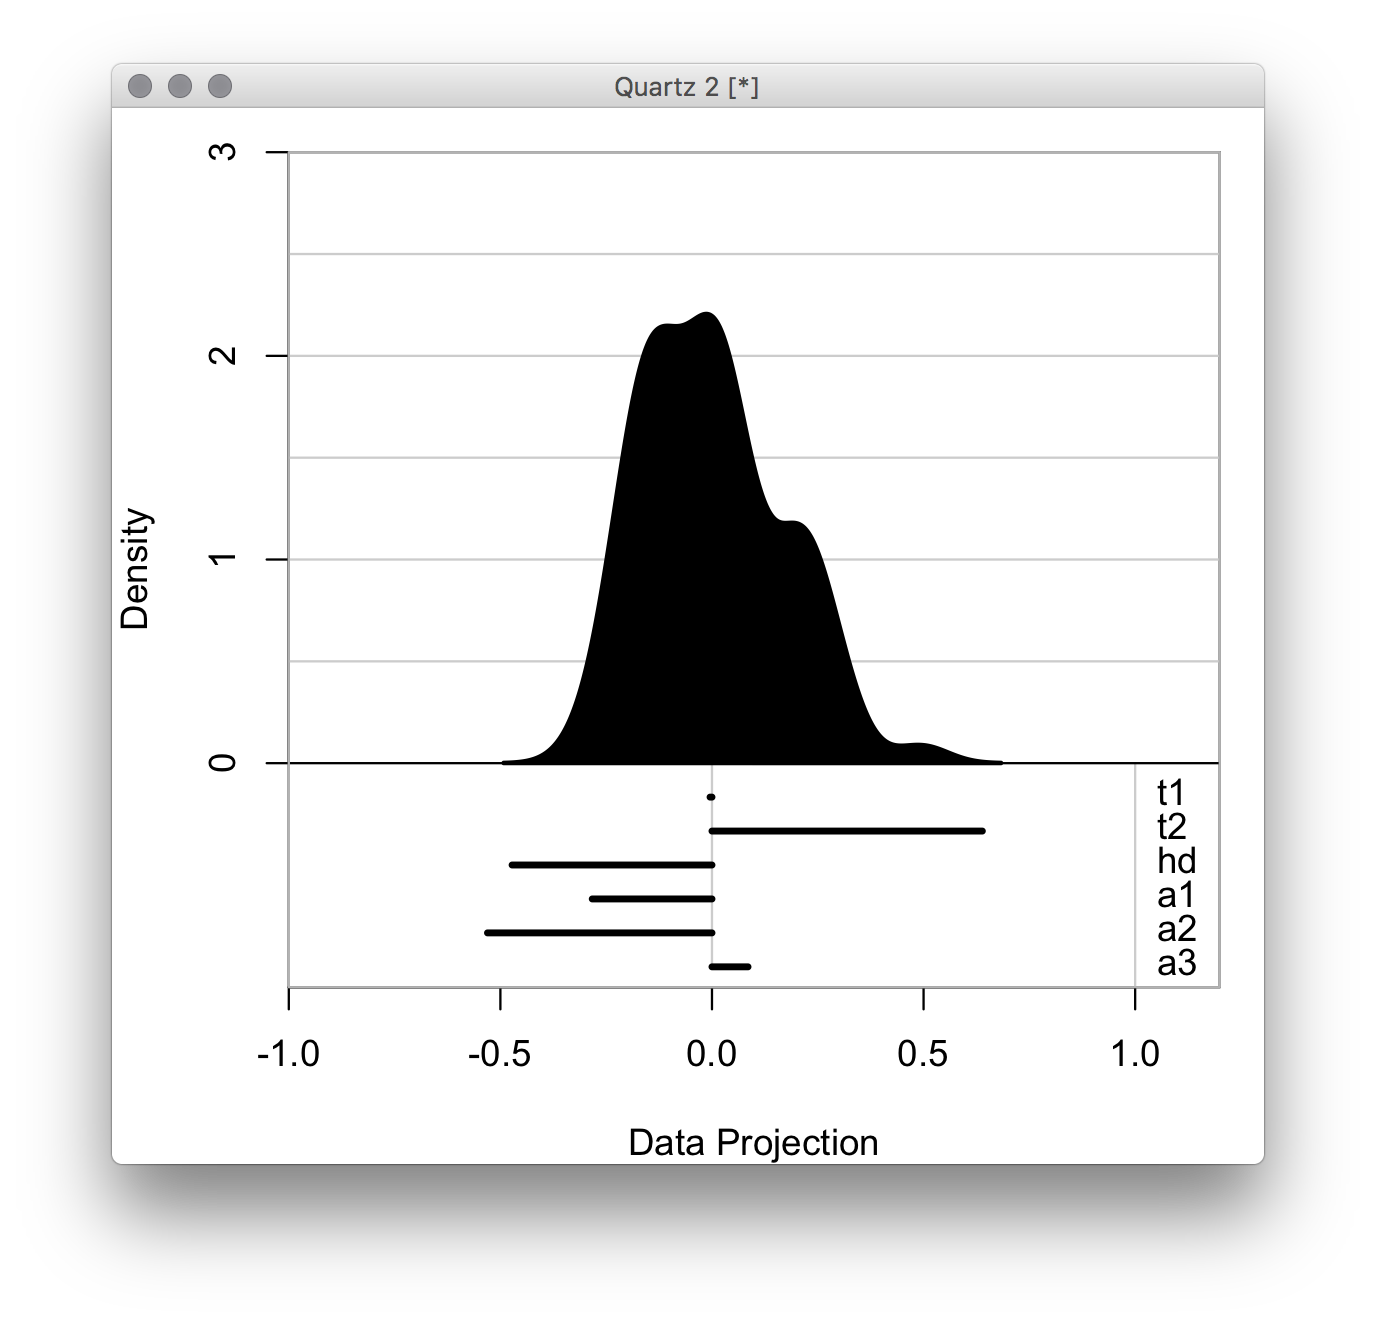
\includegraphics[width=5cm]{figures/tour3.png}}
\caption{Three projections from a 1D tour of 6D data, displayed as a density. Full video can be seen at https://vimeo.com/255466661.}
\label{tour}
\end{figure}

A tour path is a smooth sequence of projection matrices, \(p\times d\),
that when combined with a matrix of n data points, \(n\times p\), and a
rendering method, produces a steady stream of \(d\)-dimensional views of
the data. Each tour is initialised with the \texttt{new\_tour()} method,
which instantiates a tour object and takes as arguments the data \(X\),
the tour method, e.g. \texttt{guided\_tour()}, and the starting basis.
Once initialised, a new target plane is chosen, and a series of steps
along a geodesic path from starting to target plane are generated by
interpolation.

This requires a series of calls to the tour object producing the series
of projections. The steps are discrete, of size given by
\(\omega/\Delta\), where \(\omega\) denotes the angular velocity of the
geodesic interpolation, and \(\Delta\) is a parameter denoting frames
per second, reflecting the rendering speed of the device in use. The
\(\Delta\) parameter can be thought of as the frames per second, while
\(\omega\) affects the speed at which the tour moves through the
projection space. For our purposes, \(\Delta\), \texttt{fps} in the
code, is set at 25, while the \(\omega\) can be adjusted by the user.

\subsection{\texorpdfstring{Connecting the tour projections to D3
display using
\texttt{sendCustomMessage}}{Connecting the tour projections to D3 display using sendCustomMessage}}\label{connecting-the-tour-projections-to-d3-display-using-sendcustommessage}

D3.js (Data-Driven Documents) (Bostock, Ogievetsky, and Heer
\protect\hyperlink{ref-D3}{2011}) is a JavaScript library for
manipulating documents based on data. The advantages of D3 are similar
to those provided by Shiny: namely, an industry standard with rich array
of powerful, easy to use methods and widgets that can be displayed on a
wide variety of devices, with a large user base. D3 works on data
objects in the JavaScript Object Notation (JSON) format, which are then
parsed and used to display customisable data visualisations.

The new implementation of the tour interface uses D3 to render each
projection step returned by R, focusing on 2D projections as a test
case. It does this by drawing and re-drawing a scatterplot with dots (or
circles in D3 language) and providing SVG objects for the web browser to
render. Figure \ref{tourrD3} shows the new GUI.

\begin{figure*}[ht]
\centerline{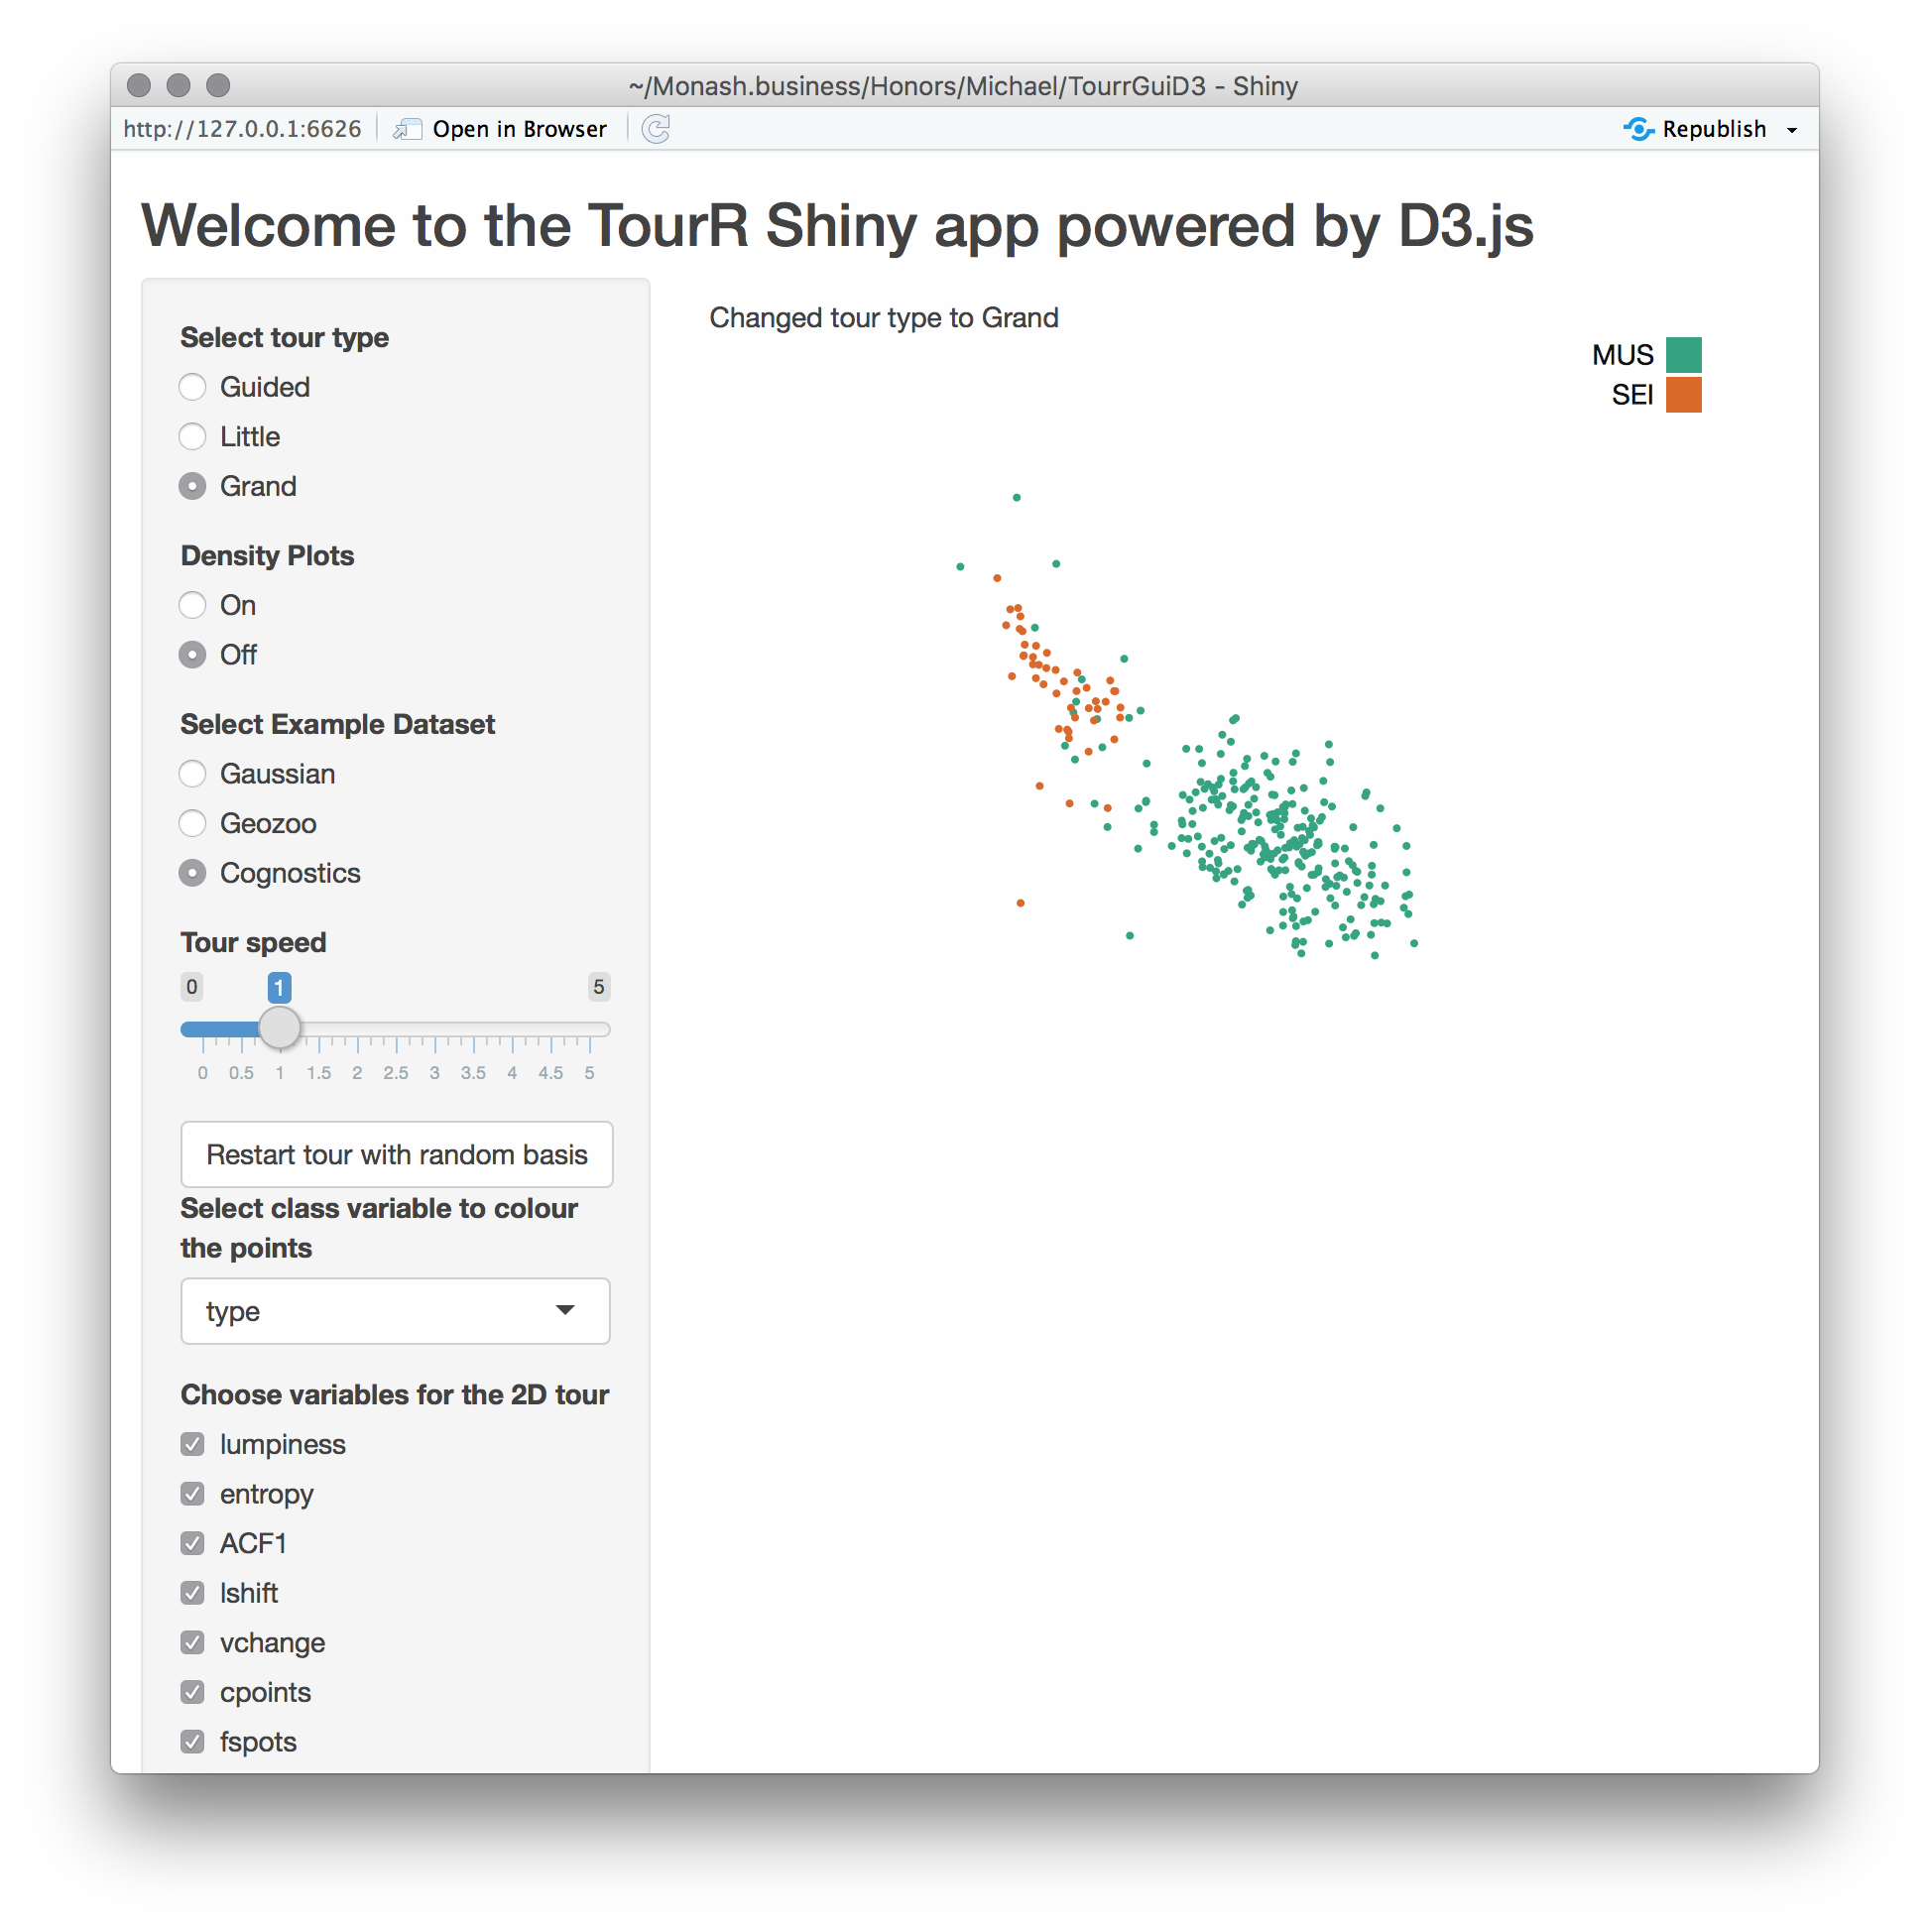
\includegraphics[width=15cm]{figures/TourrD3.png}}
\caption{Shiny GUI for the tour, with D3 as the display engine. GUI provides controls to select tour type, change speed, restart, and select variables to include.}
\label{tourrD3}
\end{figure*}

There are two functions provided by the Shiny framework to transport
data between R and JavaScript: \texttt{session\$sendCustomMessage()} in
R, and the corresponding \texttt{Shiny.addCustomMessageHandler()} in
JavaScript. Whenever the former is executed in R, the latter function
will execute a code block in JS. There are many examples of such
functions being used to pass arbitrary data from an R app to a JS
front-end, few examples exist of this basic functionality to update a D3
animation in real-time.

The data format expected by D3 is in JSON format, which combines two
basic programming paradigms: a collection of name/value pairs, and an
ordered list of values. R's preferred data formats include data frames,
vectors and matrices. Every time a new projection has been calculated
with the tour path, the resulting matrix needs to be converted to JSON
and sent to D3. The code to send the D3 data looks like this:

\begin{verbatim}
session$sendCustomMessage(type = "data", message = toJSON(j))
\end{verbatim}

This code is from the observe environment from the \texttt{server.R}
file. It converts the matrix of projected data points to JSON format,
and sends it to JavaScript with the id data. When parsed in D3 by its
\texttt{data()} method, it is converted back into a logical 2D array
where the columns are queried first, then the rows. If column names are
included in the JSON, the column indices are strings; otherwise they are
integers starting from 1. All of the code required to render the
scatterplots and legends, along with colours, is JavaScript code in the
file \texttt{d3anim.js}. In particular, the data from R is handled with
the following code:

\begin{verbatim}
Shiny.addCustomMessageHandler("data",
    function(message) {
        /* D3 scatterplot is drawn and re-drawn using the
            data sent from the server. */
}
\end{verbatim}

Every time the message is sent (25 times per second), the code-block is
run.

\subsection{Getting projections}\label{getting-projections}

The \texttt{observeEvent} Shiny method defines a code block to be run
whenever some input value changes. The following code snippet restarts a
tour using a random basis:

\begin{verbatim}
observeEvent(input$restart_random,
  {
    p <- length(input$variables)
    b <- matrix(runif(2*p), p, 2)
    rv$tour <- 
      new_tour(as.matrix(rv$d[input$variables]),
              choose_tour(input$type, 
              input$guidedIndex,
              c(rv$class[[1]]), 
              input$scagType), b)
})
\end{verbatim}

The projections are calculated using the tour object in an
\texttt{observe()} environment, which repeatedly runs the code until a
reactive variable is changed, at which point it is ``invalidated'' and
then re-started. The projections are calculated using the following code
block:

\begin{verbatim}
observe({
  tour <- rv$tour
  aps <- rv$aps
  step <- tour(aps / fps)
  if (!is.null(step)) {
    invalidateLater(1000 / fps)
    j <- center(rv$mat %*% step$proj)
    j <- cbind(j, class = rv$class)
    colnames(j) <- NULL
    session$sendCustomMessage(type = "data", 
      message = toJSON(j))
  }
  else {
    if (length(rv$mat[1, ]) < 3) {
    session$sendCustomMessage(type = "debug", 
      message = "Error: Need > 2 variables.")
    } else {
    session$sendCustomMessage(type = "debug", 
    message = "Guided tour finished: no better bases found.")
    }
  }
})
\end{verbatim}

\subsection{Pros and cons}\label{pros-and-cons}

The D3 canvas makes for smooth drawing and re-drawing of the data
projections. Adding a GUI around the display is straightforward with the
Shiny package, e.g.~control elements such as stop/go, increase/decrease
speed, change tour type, add/remove variables from the mix.

The main disadvantage is that the speed is inconsistent, as server and
client play tag to keep up with each other, and the display cannot
handle many observations. Noticeable slow down was oberved with 2000
points, the main reason being the rendering time required for the large
number of SVG circle elements. The situation can be improved when using
a single HTML5 canvas element to draw the scatter points, significantly
reducing the rendering time.

Another disadvantage is that the displays needs to be coded anew. D3
provides mostly primitives, and example code, to make scatterplots, and
contours, but the data displays all need to be coded again.

\subsection{Summary}\label{summary}

The custom message tools from Shiny provide a way to share a tour path
with the D3 renderer, and embed it in a Shiny GUI providing controls
such as stop/go, increase/decrease speed, change tour type, add/remove
variables. However, the approach doesn't provide the smooth motion that
is needed for easy display of projections, and is slow for large numbers
of observations.

\subsection{Code}\label{code}

The code is available at \url{https://github.com/makipp/TourrGuiD3}, and
the source material for this paper is available at
\url{https://github.com/dicook/paper-tourrd3}.

\subsection{Acknowledgements}\label{acknowledgements}

Thanks to Yihui Xie for pointing out the custom message tools.

\subsection{References}\label{references}

\hypertarget{refs}{}
\hypertarget{ref-D3}{}
Bostock, Michael, Vadim Ogievetsky, and Jeffrey Heer. 2011. ``D3:
Data-Driven Documents.'' \emph{IEEE Transactions on Visualization and
Computer Graphics} 17 (12): 2301--9.
\url{http://vis.stanford.edu/papers/d3}.

\hypertarget{ref-shiny}{}
Chang, Winston, Joe Cheng, JJ Allaire, Yihui Xie, and Jonathan
McPherson. 2017. \emph{Shiny: Web Application Framework for R}.
\url{https://CRAN.R-project.org/package=shiny}.

\hypertarget{ref-gt_pp}{}
Cook, Dianne, Andreas Buja, Javier Cabrera, and Catherine Hurley. 1995.
``Grand Tour and Projection Pursuit.'' \emph{Journal of Computational
and Graphical Statistics} 4 (4): 155--72.

\hypertarget{ref-gt_pp_mc}{}
Cook, Dianne, Andreas Buja, Eun-Kyung Lee, and Hadley Wickham. 2007.
``Grand Tours, Projection Pursuit Guided Tours and Manual Controls.''

\hypertarget{ref-tourrGui}{}
Huang, Bei, Dianne Cook, and Hadley Wickham. 2012. ``TourrGui: A
gWidgets Gui for the Tour to Explore High-Dimensional Data Using
Low-Dimensional Projections.'' \emph{Journal of Statistical Software} 49
(6): 1--12.

\hypertarget{ref-ihaka:1996}{}
Ihaka, Ross, and Robert Gentleman. 1996. ``R: A Language for Data
Analysis and Graphics.'' \emph{Journal of Computational and Graphical
Statistics} 5 (3): 299--314.

\hypertarget{ref-RGtk2}{}
Lawrence, Michael, and Duncan Temple Lang. 2010. ``RGtk2: A Graphical
User Interface Toolkit for R.'' \emph{Journal of Statistical Software}
37 (8): 1--52. \url{http://www.jstatsoft.org/v37/i08/}.

\hypertarget{ref-R}{}
R Core Team. 2018. \emph{R: A Language and Environment for Statistical
Computing}. Vienna, Austria: R Foundation for Statistical Computing.
\url{http://www.R-project.org/}.

\hypertarget{ref-tourr}{}
Wickham, Hadley, Dianne Cook, Heike Hofmann, and Andreas Buja. 2011.
``Tourr: An R Package for Exploring Multivariate Data with
Projections.'' \emph{Journal of Statistical Software} 40 (2): 1--18.

\address{%
Michael Kipp\\
Monash University\\
Department of Econometrics and Business Statistics\\
}
\href{mailto:mkipp271@gmail.com}{\nolinkurl{mkipp271@gmail.com}}

\address{%
Dianne Cook\\
Monash University\\
Department of Econometrics and Business Statistics\\
}
\href{mailto:dicook@monash.edu}{\nolinkurl{dicook@monash.edu}}

\address{%
Ursula Laa\\
Monash University\\
School of Physics and Astronomy\\
}
\href{mailto:ursula.laa@monash.edu}{\nolinkurl{ursula.laa@monash.edu}}

